% !TEX root = ../Group10_Assignment6_OOSC_2020.tex

\section{Frameworks}

\subsection{Actions Supported}

\begin{itemize}
	\item calculate flat size
	\begin{itemize}
		\item in the current state of SWCArchitect (that is implemented in the previous assignment), we have the 'import floorplan' function. Through that, we can get the information on the imported image, such as width and height.
		\item however, those features of width and height are abstract, they do not map to the real-world information without extra information. Due to this nature of those features, we can either:
		\begin{itemize}
			\item provide flat size in pixel$^{2}$ (e.g. height * width)
			\item we can ask for user intervention, that, at the import of floorplan, we can ask user to provide the dimensions of the flat, so we can map those real world values to the pixels. This would help us also in the other functionalities.
		\end{itemize}
		\item in the previous assignment, we have extended ImageTool to build our ImageImporter (for floorplan). This class' implementation can be used to implement this functionality of calculating flat size.
	\end{itemize}
	\bigskip
	
	\item occupied space of elements/free space
	\begin{itemize}
		\item similar to the 'calculate flat size', we can either ask for user intervention for meter$^{2}$ calculation, or even better, ask for room size once. If we have such information, then we have what is the length of each pixel in horizontal and vertical directions. With such information, we can calculate the relative size of the furnitures too.
		\item in the same sense, we implemented furnitures by extending TextAreaFigure, and we can use this to implement the given functionality.
	\end{itemize}
	\bigskip
	
	\item validate constraints, e.g. "a room has at least three connected walls"
	\begin{itemize}
		\item in the previous assignment, we also implemented some of the constraints.\\
		Citing from our own previous assignment:
		
		\begin{addmargin}[4em]{0em}
			\textit{Wall, Door and Window are extending ImageFigure. Also, Door and Window are created by a special
				CreationTool named "CreateInWallElement". It checks that doors and windows are always placed on a
				wall. If not, it intercepts the call of the framework to mousePressed.}
		\end{addmargin}
		
		\item we can use this to enforce some of the constraints. For the rest of the constraints, we would use Template-Hook approach to enable user to add more constraint by coding, if a need is deemed necessary.
	\end{itemize}
	
	\item mass operations (resizing of multiple objects)
	\begin{itemize}
		\item multiple items can be chosen \& resized.\\
			In order to allow grouping, such as:
			\begin{itemize}
				\item only group certain kind of furniture (e.g. only chairs)
				\item group more than one kind of furniture (like the example in the previous assignment: table \& chair grouping)
			\end{itemize}
	
		\item for such flexibility, we would also use one of the Template-Hook approaches, so the user-generated furniture types are also allowed to be grouped without selecting them manually.
	\end{itemize}
\end{itemize}

\subsection{UI choice}

We would like to select the first of the provided UI dialogues. Thanks to the jHotDraw support of the menu implementation, it would allow for an easier and cleaner implementation of the inclusion of additional features. A drop-down added to the menu-bar would also allow for the users to already feel comfortable with functionality that is added in an intuitive way. We believe that the second UI could confuse potential users of our application with regards to the behaviour of the added functionality.

\subsection{Framework properties and patterns}
We would like to define this framework as a white-box framework, as it will be an extension of the jHotDraw framework. We would like to propose an implementation that would allow the usage of elements such as Figures. For that to work nicely, we would like to propose the following patterns to provide support of our implementation:

\subsubsection{Calculate flat size}
For the calculation of the flat area, we would like to propose the usage of \textbf{Singleton Pattern}. We would like to additionally ask the user after they upload a background image to provide the width and height of the flat. Those could then be mapped onto the amount of pixels in width and height respectively to be able to approximate the size of each of the elements. This means that the flat size would be not only an accurate measure, but also easily accessible by all components that need it.

\subsubsection{Occupied space of elements/free space}
The calculation of the occupied space/free space would also follow a similar set of steps as the flat size, but due to various object types usage, we would like to use the \textbf{Template Method Pattern}. This would allow us to provide an abstract structure containing general methods of concepts, which we could then be made more concrete in the respective classes, which define the calculation of specific object types. The calculation of the occupied space would then simply be made by addition of the results of the helper classes. One could then obtain the free space based on the subtraction between the flat size and the above mentioned addition result.

\subsubsection{Validate constraints}
For the validation of constraints we would like to propose the \textbf{1:n Connection meta-pattern} with \textbf{Observer pattern}. Not only would we then be able to define constraints for various types of objects, but also provide a quick response to the changes made in the UI by the user. This is very important in the constraint validation. As we have various object types and various constraints that are relevant to them, the 1:n Connection seems a relatively obvious choice.
The notify in the ConstraintHolder would then be responsible for keeping track of all elements, which are managed in terms of a specific type of constraints and notifying all relevant observers if a constraint violation has been detected. ConstraintHolder contains also a list of all constraints to help in the notify process.

\subsubsection{Mass operations}
We would like to propose the usage of event listeners in each of the objects. When the user would like to for example resize all chairs in the image, they would have to emit chair resize event, which would trigger all relevant chairs to update their sizing accordingly.


\subsection{UML Diagrams}

\subsubsection{Area Calculations}

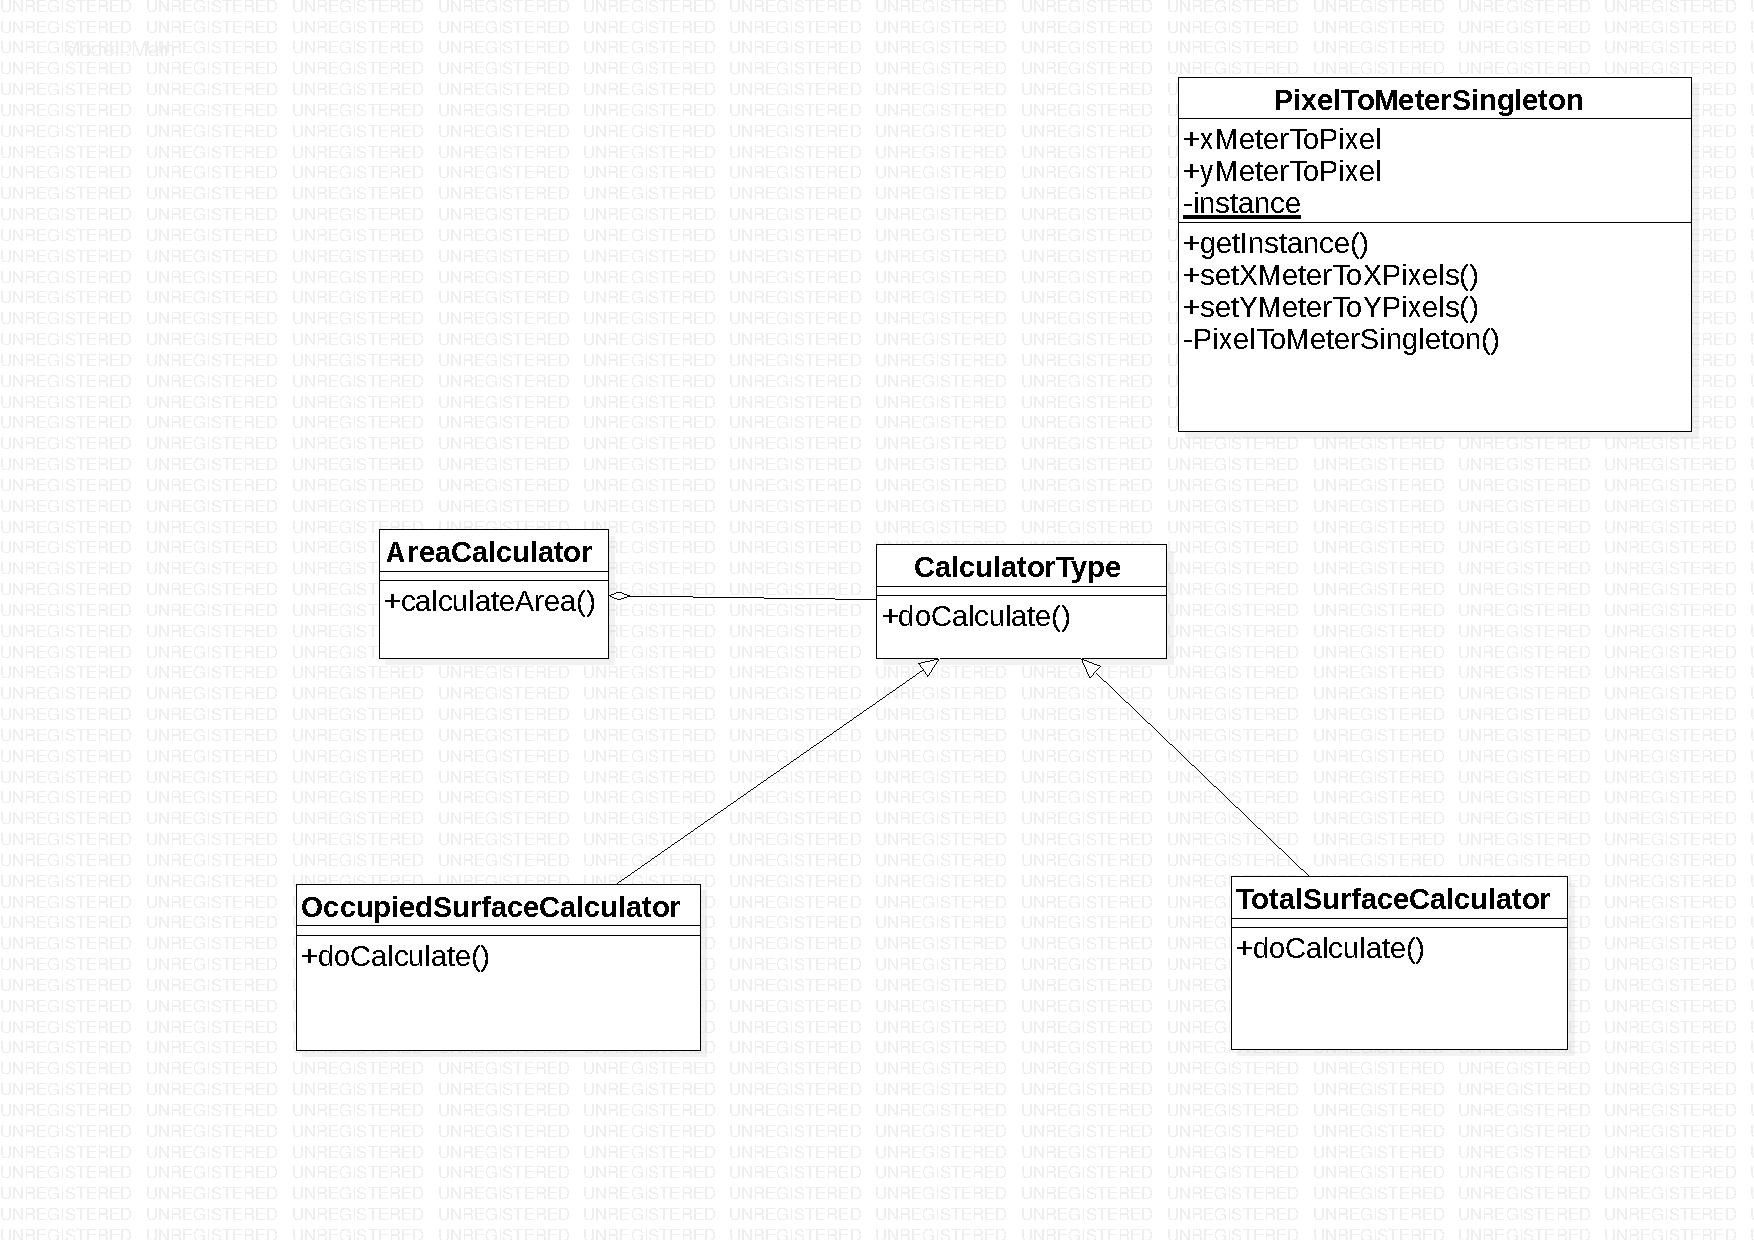
\includegraphics[width=\textwidth]{../uml/area}

\subsubsection{Constraint Validation}

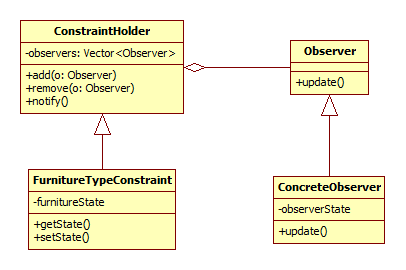
\includegraphics[width=\textwidth]{../uml/constraint.png}
